\documentclass[titlepage,a4paper,12pt]{report}
\usepackage{amssymb,amsfonts,amsmath}
\usepackage{fullpage}
\usepackage{graphicx}
%\usepackage[cc]{titlepic}
\usepackage{amsthm}
\newtheorem{definition}{Definition}[section]
\newtheorem{example}{Example}[section]
\newtheorem{theorem}{Theorem}[section]
\newtheorem{exercise}{Exercise}[section]
\newtheorem{corollary}{Corollary}[section]
\newtheorem{proposition}{Proposition}[section]
\pdfpagewidth 8.5in
\pdfpageheight 11in
\setlength\topmargin{-0.5in}
\setlength\headheight{0in}
\setlength\headsep{0in}
\setlength\textheight{9.5in}
\setlength\textwidth{7.0in}
\setlength\oddsidemargin{-0.5in}
\setlength\evensidemargin{1.0in}
\setlength\parindent{0.25in}
\setlength\parskip{0.25in}
%\begin{titlepage}
%\usepackage{titlepic}
%\titlepic{
\includegraphics[width=0.2\textwidth]{uz1.png}}
%
%\title{\textbf{HMTH111 Calculus 2}}
%\author{Nhawu. G\\
%		Department of Mathematics\\
%		University of Zimbabwe, ZIM}
%
%\end{titlepage}

\begin{document}
\begin{titlepage}
 
\begin{center}
 
 
% Upper part of the page

\includegraphics[width=0.15\textwidth]{uz1.png}\\[1cm]
 
\textsc{\LARGE University of Zimbabwe}\\[1.5cm]
 
\textsc{\Large HMTHCS111 CALCULUS 2}\\[0.5cm]
 
 
% Title

{ \huge \bfseries Calculus of Several Variables}\\[0.4cm]
 

 
% Author and supervisor
\begin{minipage}{0.4\textwidth}
\begin{center} \large
\emph{Author:}\\
G. \textsc{Nhawu}
\end{center}
\end{minipage}
\begin{minipage}{0.4\textwidth}
\begin{flushright} \large
\emph{Department:} \\
\textsc{Mathematics and Computational Sciences}
\end{flushright}
\end{minipage}

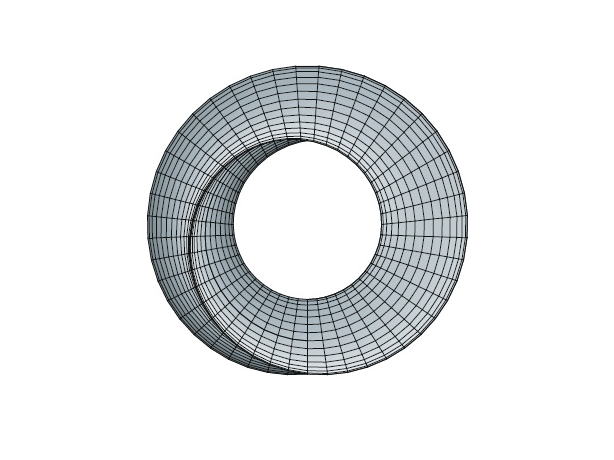
\includegraphics[width=0.7\textwidth]{umblictorus.png}\\[1cm]
 \vfill
 
 
% Bottom of the page
{\large \today}
 
\end{center}
 
\end{titlepage}
%\maketitle
\tableofcontents
\setcounter{chapter}{5}
\chapter{Functions of Several Variables}
\begin{center}
\small{\parbox{18cm}{
		\begin{raggedright}
		{\small
		\textit{Anyone who has never made a mistake has never tried anything new.}
 }
 
				\vspace{.5cm}\hfill{---Albert Einstein}
		\end{raggedright}
	}
} 
\end{center}
So far we have dealt only with functions of single (independent) variables. Many familiar quantities, however, are functions of two or more variables. For instance, the work done by a force ($W=FD$) and the volume of a right circular cylinder ($V=\pi r^2 h$) are both functions of two variables. The volume of a rectangular solid ($V=lwh$) is a function of three variables.  The notation for a function of two or three variables is as follows 
\[z=f\underbrace{(x,y)}_{2\, variables}=x^2+xy\] and \[w=f\underbrace{(x,y,z)}_{3\, variables} =x+2y-3z.\]
\section{Definition of a Function of Two Variables}
Let $D$ be a set of ordered pairs of real numbers. If to each ordered pair $(x,y)$ in $D$ there corresponds a unique real number $f(x,y)$, then $f$ is called a \textbf{function of $x$ and $y$}. The set $D$ is the \textbf{domain} of $f$ and the corresponding set of values for $f(x,y)$ is the \textbf{range} of $f$. For the function given by $z=f(x,y)$, we call $x$ and $y$ the \textbf{independent variables} and $z$ the \textbf{dependent variable}.

\noindent As with functions of one variable, the most common way to describe a function of several variables is with an \textit{equation}, and unless otherwise restricted, we can assume that the domain is the set of all points for which the equation is defined. for example, the domain of the function given by 
\[f(x,y)=x^2+y^2\] is assumed to be the entire $xy-$plane.

\begin{example}
Find the domains of the following functions.
\[(i)\, f(x,y)=\dfrac{\sqrt{x^2+y^2-9}}{x} \quad \quad \quad  (ii)\, g(x,y,z)=\dfrac{x}{\sqrt{9-x^2-y^2-z^2}}.\]

\noindent \textbf{Solution:} (i)\, The function $f$ is defined for all points $(x,y)$ such that $x\neq 0$ and $x^2+y^2\geq 9$. Thus, the domain is the set of all points lying on or outside the circle $x^2+y^2=9$.

\noindent (ii)\, The function $g$ is defined for all points $(x,y,z)$ such that $x^2+y^2+z^2<9$. Consequently, the domain is the set of all points $(x,y,z)$ lying inside a sphere of radius $3$ that is centred at the origin.
\end{example}

\noindent Functions of several variables can be combined in the same ways as functions of single variables. For instance, we can form the sum, difference, product and quotients of two functions of two variables as follows 
\begin{enumerate}
\item $(f\pm g)(x,y)=f(x,y)\pm g(x,y)$ \quad Sum or Difference.
\item $(fg)(x,y)=f(x,y)g(x,y)$ \quad \quad ~~~~  Product.
\item $\dfrac{f}{g}(x,y)=\dfrac{f(x,y)}{g(x,y)}, \quad g(x,y)\neq 0$ \quad Quotient.
\end{enumerate}
\section{The Graph of a Function of Two Variables}
As with functions of single variables, we can learn a lot about the behaviour of a function of two variables by sketching its graph. The \textbf{graph} of a function $f$ of two variables is the set of all points $(x,y,z)$ for which $z=f(x,y)$ and $(x,y)$ is in the domain of $f$. The graph can be interpreted as a \textbf{surface in space}.
\subsection{Level Curves}
A second way to visualize a function of two variables is to use a \textbf{scalar field} in which the scalar $z=f(x,y)$ is assigned to the point $(x,y)$. A scalar field can be characterized by \textbf{level curves} (or \textbf{contour lines}) along which the value of $f(x,y)$ is constant. For example, the weather map shows level curves of equal pressure called \textbf{isobars}. In weather maps for which the level curves represent points of equal temperature, the level curves are called \textbf{isotherms}. Another common use of level curves is in representing electrical potential fields, in this type of map, the level curves are called \textbf{equipotential lines}.
\subsection{Level Surfaces}
The concept of a level curve can be extended by one dimension to define a \textbf{level surface}. If $f$ is a function of three variables and $c$ is a constant, then the graph of the equation $f(x,y,z)=c$ is a \textbf{level surface} of the function $f$.
\section{Limits and Continuity}
\subsection{Neighborhoods in the Plane}
In this section, we will study limits and continuity involving functions of two or three variables. We begin our discussion of the limit of a function of two variables by defining a two-dimensional analog to an interval on the real line. Using the formula for the distance between two points $(x,y)$ and $(x_0, y_0)$ in the plane, we can define the \textbf{$\delta$-neighborhood} about $(x_0,y_0)$ to be the \textbf{disc} centered at $(x_0,y_0)$ with radius $\delta >0$
\[\{(x,y): \sqrt{(x-x_0)^2+(y-y_0)^2}< \delta\}.\] 
\textbf{closed}.
\begin{figure}[h!]
\input{open.pic}
\caption{A closed disc}
\end{figure}
When this formula contains the \textit{less than} inequality, $<$, the disc is called \textbf{open}, and when it contains the \textit{less than or equal to} inequality, $\leq$, the disc is called \textbf{closed}. 

\noindent A point $(x_0, y_0)$ in a plane region $R$ is an \textbf{interior point} of $R$ if there exists a $\delta$-neighborhood about $(x_0, y_0)$ that lies entirely in $R$. If every point in $R$ is an interior point, then $R$ is an \textbf{open region}. A point $(x_0, y_0)$ is a \textbf{boundary point} of $R$ if every open disc centered at $(x_0, y_0)$ contains points inside $R$ and points outside $R$. If a region contains all its boundary points, then the region is \textbf{closed}.
\subsection{Limit of a Function of Two Variables}
Let $f$ be a function of two variables defined on an open disc centered at $(x_0,y_0)$, except possibly at $(x_0, y_0)$ and let $L$ be a real number. Then 
\[\lim _{(x,y)\rightarrow (x_0, y_0)}f(x,y)=L\] if for each $\varepsilon >0$ there corresponds a $\delta >0$ such that 
\[|f(x,y)-L|<\varepsilon \quad {\mbox{whenever}}\quad 0<\sqrt{(x-x_0)^2+(y-y_0)^2}<\delta.\]\\
\noindent \textbf{Definition}\\
A function $f(x,y)$ has a limit $L$ as $(x,y)$ approaches $(x_0,y_0)$ if given any $\epsilon>0$ there exists \\$\delta>0$ (depending on $\epsilon$ and $(x_0,y_0)$) such that whenever $(x-x_0)^2+(y-y_0)^2<\delta^2$, then \\$|f(x,y)-L|<\epsilon$.\\~\\
\noindent The definition of the limit of a function of two variables is similar to the definition of the limit of a function of a single variable, yet there is a critical difference. For a function of two variables, the statement $(x,y)\rightarrow (x_0,y_0)$ means that the point $(x,y)$ is allowed to approach $(x_0,y_0)$ from any direction. If the value of \[\lim _{(x,y)\rightarrow (x_0,y_0)}f(x,y)\] is not the same for all possible approaches or \textbf{paths}, to $(x_0,y_0)$, then the limit does not exist. We usually choose convenient paths. Some of these are 
 \begin{enumerate}
 \item along the $x$ or $y$ axis,
 \item along straight lines, 
 \item along well-defined curves such as parabolae, for e.g.,  $y=x^3$.
 \end{enumerate}
 
 \begin{example}
 Show that \[\lim _{(x,y)\rightarrow (a,b)}x =a.\] 
 
 \noindent \textbf{Solution:} Let $f(x,y)=x$ and $L=a$. We need to show that for each $\varepsilon >0$, there exists a $\delta-$neighborhood about $(a,b)$ such that 
 \[|f(x,y)-L| =|x-a|<\varepsilon\] whenever $(x,y)\neq (a,b)$ lies in the neighborhood. We can observe that from \[0<\sqrt{(x-a)^2+(y-b)^2}<\delta\] it follows that 
 \[|f(x,y)-a|=|x-a|=\sqrt{(x-a)^2}\leq \sqrt{(x-a)^2+(y-b)^2}<\delta.\] thus, we can choose $\delta = \varepsilon$, and the limit is verified.
 \end{example}
 \begin{example}
 Prove that $\displaystyle \lim _{(x,y)\rightarrow (1,2)}x^2+2y=5$.
 
 \noindent \textbf{Solution:} Using the definition of limits, we must show that, given $\varepsilon >0$, we can find a $\delta >0$ such that $|x^2+2y-5|<\varepsilon$ when $0<|x-1|<\delta$ and $0<|y-2|<\delta$. If $0<|x-1|<\delta$ and $0<|y-2|<\delta$, then 
 \[1-\delta <x<1+\delta\] and \[2-\delta <y<2+\delta\] excluding $x=1$ and $y=2$. Thus, 
 \[1-2\delta +\delta ^2 <x^2<1+2\delta +\delta ^2\] and \[4-2\delta <2y<4+2\delta.\]
 Adding 
 \[5-4\delta +\delta ^2 <x^2+2y <5+4\delta +\delta ^2\] or 
 \[-4\delta +\delta ^2 <x^2+2y-5<4\delta +\delta ^2.\] If $\delta \leq 1$, it follows that 
 \[-5\delta<x^2+2y-5<5\delta\] i.e., $|x^2+2y-5|<5\delta$ whenever $0<|x-1|<\delta$ and $0<|y-2|<\delta$. Choosing $5\delta =\varepsilon$ i.e., $\delta =\frac{\varepsilon}{5}$ or $\delta =1$ which ever is smaller, it follows that $|x^2+2y-5|<\varepsilon$ when $0<|x-1|<\delta$ and $0<|y-2|<\delta$ i.e., $\displaystyle \lim _{(x,y)\rightarrow (1,2)}x^2+2y=5$.
 \end{example}
 \begin{example}
 Show that the following limit does not exist.
 \[\lim _{(x,y)\rightarrow (0,0)}\left(\dfrac{x^2-y^2}{x^2+y^2}\right)^2.\]
 
 \noindent \textbf{Solution:}  The domain of the function given by $f(x,y)=\left(\dfrac{x^2-y^2}{x^2+y^2}\right)^2$ consists of all points in the $xy$-plane except for the point $(0,0)$. To show that the limit as $(x,y)$ approaches $(0,0)$ does not exist, consider approaching $(0,0)$ along two different paths. along the $x$-axis, every point is of the form $(x,0)$ and the limit along this approach is 
 \[\lim _{(x,0)\rightarrow (0,0)}\left(\dfrac{x^2-y^2}{x^2+y^2}\right)^2 =\lim _ {(x,0)\rightarrow (0,0)}(1)^2=1.\] However, if $(x,y)$ approaches $(0,0)$ along the line $y=x$, we obtain 
 \[\lim _{(x,x)\rightarrow (0,0)}\left(\dfrac{x^2-y^2}{x^2+y^2}\right)^2 =\lim _{(x,x)\rightarrow (0,0)}\left(\dfrac{0}{2x^2}\right)^2=0. \] Hence, $f $does not have a limit as $(x,y)\rightarrow (0,0)$.
 \end{example}
 \begin{example}
 Show that $\displaystyle \lim _{(x,y)\rightarrow (0,0)}\dfrac{xy}{x^2+y^2}$ does not exist.
 
 \noindent \textbf{Solution:} The fact that the limit taken along the $x$ and $y-$axis exists and equal zero may lead us to suspect that the $\displaystyle \lim _{(x,y)\rightarrow (0,0)}f(x,y)$ exists. We have not examined every path to $(0,0)$. We now try any line through the origin given by $y=mx$, 
 \[\lim _{(x,y)\rightarrow (0,0)}f(x,y)=\lim _{(x,y)\rightarrow (0,0)}\dfrac{mx^2}{x^2+m^2x^2}=\dfrac{m}{1+m^2}.\]
 This limit changes as the gradient $m$ changes. For example (i)\, on $y=2x, \displaystyle \lim _{(x,y)\rightarrow (0,0)}f(x,y)=\dfrac{2}{5}$ and (ii)\, on $y=5x, \displaystyle \lim _{(x,y)\rightarrow (0,0)}f(x,y)=\dfrac{5}{26}$. There is no single number $L$ that we can call the limit of $f$ as $(x,y)\rightarrow (0,0)$. So the limit does not exist.
  \end{example}
 \subsection{Limit Combinations}
 In general, if $\displaystyle \lim _{(x,y)\rightarrow (x_0,y_0)}f(x,y)=L_1$ and $\displaystyle \lim _{(x,y)\rightarrow (x_0,y_0)}g(x,y)=L_2$, then 
 \begin{enumerate}
 \item $\displaystyle \lim [f(x,y)\pm g(x,y)]=\lim f(x,y)\pm\lim g(x,y)=L_1\pm L_2$.
 \item $\displaystyle \lim [f(x,y)\cdot g(x,y)]=(\lim f(x,y))(\lim g(x,y))=L_1L_2$.
 \item $\displaystyle \lim cf(x,y)=c\lim f(x,y)=cL_1$, where $c$ is any number.
 \item $\displaystyle \lim \dfrac{f(x,y)}{g(x,y)}=\dfrac{\lim f(x,y)}{\lim g(x,y)}=\dfrac{L_1}{L_2}$, if $L_2\neq 0$.
 \end{enumerate}
 \begin{example}
 Evaluate $\displaystyle \lim _{(x,y)\rightarrow (2,1)}(2x+5xy-3y^2)$.
 
 \noindent \textbf{Solution:} \begin{eqnarray*}
 \lim _{(x,y)\rightarrow (2,1)} (2x+5xy-3y^2) &=&  \lim _{(x,y)\rightarrow (2,1)} 2x + \lim _{(x,y)\rightarrow (2,1)} 5xy + \lim _{(x,y)\rightarrow (2,1)} (-3y^2)\\
 &=& \lim _{x\rightarrow 2} 2x + (\lim _{x\rightarrow 2} 5x)(\lim _{y\rightarrow 1}y)-3\lim _{y\rightarrow 1} y^2 \\
 &=& 2\lim _{x\rightarrow 2} x +5(\lim _{x\rightarrow 2}x)(\lim _{y\rightarrow 1}y)-3(\lim _{y\rightarrow 1}y)(\lim _{y\rightarrow 1}y)\\
 &=& 2 \cdot 2 +5\cdot 2 \cdot 1-3\cdot 1\cdot 1 =4+10-3=11.
 \end{eqnarray*}
 \end{example}
 \section{Continuity of a Function of Two Variables}
 Notice that the limit of 
 \[f(x,y)=\dfrac{5x^2y}{x^2+y^2}\] as $(x,y)\rightarrow (1,2)$ can be evaluated by direct substitution. That is, the limit is $f(1,2)=2$. In such cases the function $f$ is said to be \textbf{continuous} at the point $(1,2)$.
 \subsubsection{Definition of Continuity of a Function of Two Variables}
 A function $f$ of two variables is \textbf{continuous at a point $(x_0,y_0)$} in an open region $R$ if
 \begin{enumerate}
 \item $f$ is defined at $(x_0,y_0)$,
 \item $\displaystyle \lim _{(x,y)\rightarrow (x_0,y_0)}f(x,y)$ exists, and 
 \item $\displaystyle \lim _{(x,y)\rightarrow (x_0,y_0)}f(x,y)=f(x_0,y_0).$
\end{enumerate}  
$f(x_0,y_0)$ is equal to the limit of $f(x,y)$ as $(x,y)$ approaches $(x_0,y_0)$, i.e., 
 \[\lim _{(x,y)\rightarrow (x_0,y_0)}f(x,y)=f(x_0,y_0).\] 
 The function $f$ is \textbf{continuous in the open region $R$} if it is continuous at every point in $R$.
 \subsubsection{Properties of Continuous Functions of Two Variables}
 If $k$ is a real number and $f$ and $g$ are continuous at $(x_0,y_0)$, then the following functions are continuous at $(x_0,y_0)$, 
 \begin{enumerate}
 \item Scalar Multiple $kf$.
 \item Sum and difference $f\pm g$. 
 \item Product $fg$.
 \item Quotient $\dfrac{f}{g}$, if $g(x_0,y_0)\neq 0$.
 \end{enumerate}
 Polynomials and rational functions in two variables are continuous at any point at which they are defined.
\section{Partial Derivatives}
\subsection{Partial Derivatives of a Function of Two Variables}
In the application of functions of several variables, the question often arises, ``How will a function be affected by a change in one of its independent variables?''. You can answer by considering the independent variables one at a time.  The process is called \textbf{partial differentiation}, and the result is referred to as the \textbf{partial derivative} of $f$ with respect to the chosen independent variable \footnote{The introduction of partial derivatives followed Newton's and Leibniz's work in calculus by several years. Between 1760, Leonhard Euler and Jean Le Rond d'Alembert (1717-1783) separately published several papers on dynamics, in which they established much of the theory of partial derivatives}. 
\subsubsection{Definition of Partial Derivatives of a Function of Two Variables }
If $z=f(x,y)$, then the \textbf{first partial derivatives} of $f$ with respect to $x$ and $y$ are the functions $f_x$ and $f_y$ defined by 
\begin{eqnarray*}
f_x(x,y) &=& \lim _{\Delta x \rightarrow 0} \dfrac{f(x+\Delta x,y)-f(x,y)}{\Delta x}\\
f_y(x,y) &=& \lim _{\Delta y \rightarrow 0} \dfrac{f(x,y+\Delta y)-f(x,y)}{\Delta y}
\end{eqnarray*}
provided the limits exist.
This definition indicates that if $z=f(x,y)$, then to find $f_x$ we \textit{consider $y$ constant and differentiate with respect to $x$}. Similarly, to find $f_y$, we \textit{consider $x$ constant and differentiate with respect to $y$}.
\begin{example}
Find $f_x$ and $f_y$ for $f(x,y)=3x-x^2y^2+2x^3y$.

\noindent \textbf{Solution:} Considering $y$ to be constant and differentiating with respect to $x$ produces 
\[f_x(x,y)=3-2xy^2+6x^2y.\]
Considering $x$ to be constant and differentiating with respect to $y$ produces
\[f_y(x,y)=-2x^2y+2x^3.\]
\end{example}
 \subsubsection{Notation for Partial Derivatives}
For $z=f(x,y)$, the partial derivatives $f_x$ and $f_y$ are denoted by 
\[\dfrac{\partial }{\partial x} f(x,y)=f_x(x,y)=z_x=\dfrac{\partial z}{\partial x}\] and 
\[\dfrac{\partial }{\partial y} f(x,y)=f_y(x,y)=z_y=\dfrac{\partial z}{\partial y}.\] 
The first partials evaluated at the point $(a,b)$ are denoted by 
\[\dfrac{\partial z}{\partial x}\Biggl |_{(a,b)}=f_x(a,b)\] and 
\[\dfrac{\partial z}{\partial y}\Biggl |_{(a,b)}=f_y(a,b).\]
\begin{example}
For $f(x,y)=xe^{x^2y}$, find $f_x$ and $f_y$ and evaluate each at the point $(1, \ln 2)$.

\noindent \textbf{Solution:} Because 
\[f_x(x,y)=xe^{x^2y}(2xy)+e^{x^2y}\] the partial derivative of $f$ with respect to $x$ at $(1,\ln 2)$ is 
\[f_x(1,\ln 2)=e^{\ln 2}(2\ln 2)+e^{\ln 2}=4\ln 2 +2.\]
Because 
\[f_y(x,y)=xe^{x^2y}(x^2)=x^3e^{x^2y}\] the partial derivative of $f$ with respect to $y$ at $(1,\ln 2)$ is 
\[f_y(1,\ln 2)=e^{\ln 2}=2.\]
\end{example}
\subsection{Partial Derivatives of a function of Three or More Variables}
The concept of a partial derivative can be extended naturally to functions of three or more variables. For instance, if $w=f(x,y,z)$, then there are three partial derivatives, each of which is formed by holding two of three variables constant.
\begin{eqnarray*}
\dfrac{\partial w}{\partial x} &=& f_x(x,y,z)=\lim _{\Delta x \rightarrow 0} \dfrac{f(x+\Delta x, y, z)-f(x,y,z)}{\Delta x} \\
\dfrac{\partial w}{\partial y} &=& f_y(x,y,z)=\lim _{\Delta y \rightarrow 0} \dfrac{f(x,y+\Delta y, z)-f(x,y,z)}{\Delta y} \\
\dfrac{\partial w}{\partial z} &=& f_z(x,y,z)=\lim _{\Delta z \rightarrow 0} \dfrac{f(x,y,z+\Delta z)-f(x,y,z)}{\Delta z}.
\end{eqnarray*}
\begin{example}
\begin{itemize}
\item[(i)] To find the partial derivative of $f(x,y,z)=xy+yz^2+xz$ with respect to $z$, consider $x$ and $y$ to be constant and obtain 
\[\dfrac{\partial}{\partial z}\left[xy+yz^2+xz\right]=2yz+x.\]
\item[(ii)] to find the partial derivative of $f(x,y,z)=z\sin (xy^2+2z)$ with respect to $z$, consider $x$ and $y$ to be constant. Then, using the Product rule, we obtain
\begin{eqnarray*}
\dfrac{\partial}{\partial z}\left[z\sin (xy^2+2z)\right] &=& (z)\dfrac{\partial}{\partial z}[\sin (xy^2+2z)] +\sin (xy^2+2z)\dfrac{\partial}{\partial z} [z]\\
&=& (z)[\cos (xy^2+2z)](2) +\sin (xy^2+2z)\\
&=& 2z\cos (xy^2+2z)+\sin (xy^2+2z).
\end{eqnarray*}
\item[(iii)] To find the partial derivative of $f(x,y,z,w)=\dfrac{x+y+z}{w}$ with respect to $w$, consider $x,y$ and $z$ to be constant and obtain
\[\dfrac{\partial }{\partial w}\left[\dfrac{x+y+z}{w}\right]=-\dfrac{x+y+z}{w^2}.\]
\end{itemize}
\end{example}
\subsection{Higher-Order Partial Derivatives}
It is possible to take second, third and higher partial derivatives of a function of several variables, provided such derivatives exist. Higher-order derivatives are denoted by the order in which the differentiation occurs. For instance, the function $z=f(x,y)$ has the following second partial derivatives.
\begin{enumerate}
\item Differentiate twice with respect to $x$:
\[\dfrac{\partial}{\partial x}\left(\dfrac{\partial f}{\partial x}\right) =\dfrac{\partial ^2 f}{\partial x^2}=f_{xx}.\]
\item Differentiate twice with respect to $y$:
\[\dfrac{\partial}{\partial y}\left(\dfrac{\partial f}{\partial y}\right) =\dfrac{\partial ^2 f}{\partial y^2}=f_{yy}.\]
\item Differentiate first with respect to $x$ and then with respect to $y$:
\[\dfrac{\partial}{\partial y}\left(\dfrac{\partial f}{\partial x}\right) =\dfrac{\partial ^2 f}{\partial y \partial x}=f_{xy}.\]
\item Differentiate first with respect to $y$ and then with respect to $x$:
\[\dfrac{\partial}{\partial x}\left(\dfrac{\partial f}{\partial y}\right) =\dfrac{\partial ^2 f}{\partial x \partial y}=f_{yx}.\]
\end{enumerate}
The third and fourth cases are called \textbf{mixed partial derivatives}.
\begin{example}
Find the second partial derivatives of $f(x,y)=3xy^2-2y+5x^2y^2$ and determine the value of $f_{xy}(-1,2)$.

\noindent \textbf{Solution:} Begin by finding the first partial derivatives with respect to $x$ and $y$.
\[f_x(x,y)=3y^2+10xy^2 \quad \mbox{and}\quad f_y(x,y)=6xy-2+10x^2y.\]
Then, differentiate each of these with respect to $x$ and $y$.
\[f_{xx}(x,y)=10y^2, \quad f_{yy}(x,y)=6x+10x^2, \quad f_{xy}(x,y)=6y+20xy \quad \mbox{and} \quad f_{yx}(x,y)=6y+20xy.\] At $(-1,2)$, the value of $f_{xy}$ is $f_{xy}(-1,2)=12-40=-28$.
\end{example}
\noindent Notice that the two mixed partials are equal.  Sufficient conditions for this occurrence are given in the next theorem.
\begin{theorem}[Equality of Mixed Partial Derivatives]
If $f$ is a function of $x$ and $y$ such that $f_x$ and $f_y$ are continuous on an open disc $R$, then for every $(x,y)$ in $R$, 
\[f_{xy}(x,y)=f_{yx}(x,y).\]
\end{theorem}
\noindent The order of differentiation of the mixed partial derivatives is irrelevant. 
\begin{example}
Show that $f_{xz}=f_{zx}$ and $f_{xzz}=f_{zxz}=f_{zzx}$ for the function given by 
\[f(x,y,z)=ye^x+x\ln z.\]

\noindent \textbf{Solution:} First partials:
\[f_x(x,y,z)=ye^x+\ln z, \quad f_z(x,y,z)=\dfrac{x}{z}.\]
Second partials: (Note the first two are equal)
\[f_{xz}(x,y,z)=\dfrac{1}{z}, \quad f_{zx}(x,y,z)=\dfrac{1}{z}, \quad f_{zz}(x,y,z)=-\dfrac{x}{z^2}.\]
Third partials: (Note that all three are equal)
\[f_{xzz}(x,y,z)=-\dfrac{1}{z^2}, \quad f_{zxz}(x,y,z)=-\dfrac{1}{z^2}, \quad f_{zzx}(x,y,z)=-\dfrac{1}{z^2}.\]
\end{example}
\section{Tutorial Questions}
\begin{enumerate}
\item If $f(x,y)=x^3-2xy+3y^2$, find (i)\, $f(-2,3)$ \quad (ii)\, $f\left(\dfrac{1}{x}, \dfrac{2}{y}\right)$.
\item Give the domain for which each of the following functions is defined and is real.\\
(i)\, $f(x,y)=\dfrac{1}{x^2+y^2-1}$ \quad (ii)\, $f(x,y)=\ln (x+y)$ \quad (iii)\, $f(x,y)=\sin ^{-1}\left(\dfrac{2x-y}{x+y}\right)$ \\ (iv)\, $f(x,y)=\ln \{(16-x^2-y^2)(x^2+y^2-4)\}$ \quad (v)\, $f(x,y)=\sqrt{6-(2x+3y)}$.
\item Find the first partial derivatives with respect to $x,y$ and $z$.\\
(i)\, $w=\sqrt{x^2+y^2+z^2}$ \quad (ii)\, $w=\dfrac{xy}{x+y+z}$ \quad (iii)\, $F(x,y,z)=\ln (\sqrt{x^2+y^2+z^2})$.
\item Use the definition of a limit to show that:\\ (i)\,$\displaystyle \lim _{(x,y)\rightarrow (4,-1)}(3x-2y)=14$ \, (ii) $\displaystyle \lim _{(x,y)\rightarrow (2,1)}(xy-3x+4)=0$ \, (iii) $\displaystyle \lim _{(x,y)\rightarrow (2,1)}(2x+5xy-3y^2)=11$.
\item Let \[f(x,y) = \left\{ 
\begin{array}{l l}
 \dfrac{xy^2}{x^2+y^2}, & \quad (x,y)\neq (0,0)\\
  0, & \quad (x,y)=(0,0),\\ \end{array} \right. \]\\
Prove that $\displaystyle \lim _{(x,y)\rightarrow (0,0)}f(x,y)=0$.
\item Use rules of limits to evaluate each of the following limits.\\
(i)\, $\displaystyle \lim _{(x,y)\rightarrow (2,-1)}(3x^3-2xy+4y^2)$ \quad (ii)\, $\displaystyle \lim _{(x,y)\rightarrow (1,2)}\dfrac{3-x+y}{4+x-2y}$ \quad (iii)\, $\displaystyle \lim _{(x,y)\longrightarrow (4,\pi)}x^2\sin \left(\dfrac{y}{x}\right)$ \\ (iv)\, $\displaystyle \lim _{(x,y)\rightarrow (0^+, 1^-)}\dfrac{x+y-1}{\sqrt{x}-\sqrt{1-y}}$.
\item Show that the following limits do not exist:\\
(i)\, $\displaystyle \lim _{(x,y)\rightarrow (0,0)}\dfrac{x^2-3y^2}{x^2+2y^2}$ \quad (ii)\, $\displaystyle \lim _{(x,y)\rightarrow (0,0)}\dfrac{xy}{x^2+y^2}$ \quad (iii)\, $\displaystyle \lim _{(x,y)\rightarrow (0,0)}\dfrac{x^{2}y}{x^4+y^2}$ \quad (iv)\, $\displaystyle \lim _{(x,y)\rightarrow (0,0)}\dfrac{2x-y^2}{2x^2+y}$.
\item Use the definition of partial derivative to find $\displaystyle\frac{\partial z}{\partial x}$ and $\displaystyle\frac{\partial z}{\partial y}$ for $z=3x^2-xy+2y^2+3$.
\item If $f(x,y)=\dfrac{x-y}{x+y}$, find $\dfrac{\partial f}{\partial x}$ and $\dfrac{\partial f}{\partial y}$ from the definition.
\item Let $f(x,y)=xe^{x^2+2y^2}$, find $\dfrac{\partial f}{\partial x}$, $\dfrac{\partial f}{\partial y}$ and verify that $\dfrac{\partial^2f}{\partial x \partial y}=\dfrac{\partial^2f}{\partial y \partial x}$.
\item If $z=x^2\tan ^{-1}\dfrac{y}{x}$, find $\dfrac{\partial ^2 z}{\partial x \partial y}$ at $(1,1)$.
\item Let $f(x,y,z)=\dfrac{1}{\sqrt{x^2+y^2+z^2}}$. Show that $f_{xx}+f_{yy}+f_{zz}=0$.
\item Show that $f_x(0,0)$ and $f_y(0,0)$ exist but $f$ is not differentiable at $(0,0)$ for the following functions.\\
(i)\, $f(x,y) = \left\{ 
\begin{array}{l l}
  \dfrac{3x^2y}{x^4+y^2}, & \quad (x,y)\neq (0,0)\\
  0, & \quad (x,y)=(0,0),\\ \end{array} \right. $ \quad (ii)\, 
  $ f(x,y) = \left\{ 
\begin{array}{l l}
  \dfrac{2x^2y^2}{x^4+y^4}, & \quad (x,y)\neq (0,0)\\
  0, & \quad (x,y)=(0,0),\\ \end{array} \right. $
\item Let $$f(x,y)=\left\{\begin{array}{cc}xy\bigg(\dfrac{x^2-y^2}{x^2+y^2}\bigg)&(x,y)\neq (0,0)\cr 0&(x,y)=(0,0)\end{array} \right.$$
\begin{enumerate}
\item Show that $f(x,y)$ is continuous at the origin.
\item Find $f_{x}(0,0)$ and $f_{y}(0,0).$
\item Compute $f_{x}(x,y)$ and $f_{y}(x,y)$ where $(x,y)\neq(0,0)$.
\item Find $f_{xy}(0,0)$ and $f_{yx}(0,0)$ and verify that $f_{xy}(0,0)\neq f_{yx}(0,0)$.
\end{enumerate}
\item Find $\dfrac{dw}{dt}$ given that (i)\, $w=x^2+y^2, x=e^t, y=e^{-t}$ \quad (ii)\, $w=\ln \left(\dfrac{y}{x}\right), x=\cos t, y=\sin t$\\
(iii), $w=\sqrt{x^2+y^2}, x=\sin t, y=e^t$.
\item Find $\dfrac{\partial r}{\partial x}, \, \dfrac{\partial r}{\partial y}$ and $\dfrac{\partial r}{\partial z}$.\\
  (i)\, $r=e^{u+v+w}$ and $u=yz, \, v=xz, \, w=xy$ (ii)\, $r=uvw-u^2-v^2-w^2$ and $u=y+z, \\ v=x+z, \, w=x+y$.
\item Let $f(x,y)$ be a function of $x$ and $y$ where $x=e^{u-v}\mbox{cos}(u+v)$, $y=e^{u-v}\mbox{sin}(u+v)$.\\
Show that \begin{equation*}
\frac{\partial f}{\partial u}+\frac{\partial f}{\partial v}=2x\frac{\partial f}{\partial y}-2y\frac{\partial f}{\partial x}.
\end{equation*}
\item Assume that $w=f(u,v)$ where $u=x+y$ and $v=x-y$. Show that 
  \[\dfrac{\partial w}{\partial x}\dfrac{\partial w}{\partial y}=\left(\dfrac{\partial w}{\partial u}\right)^2-\left(\dfrac{\partial w}{\partial v}\right)^2.\]
\item Suppose that $w=f(x,y)$ and that $x=u+v$ and $y=u-v$. Show that 
\begin{equation*}
\dfrac{\partial ^2 w}{\partial x^2}-\dfrac{\partial ^2 w}{\partial y^2}=\dfrac{1}{2}\bigg(\dfrac{\partial ^2 w}{\partial u\partial v}+\dfrac{\partial ^2 w}{\partial v\partial u}\bigg).
\end{equation*}
\item Let $V=f(x,y)$, where $x$ and $y$ are given in polar co-ordinates by the equations $x=r\cos \theta$ and $y=r\sin \theta$. Show that $\left(\dfrac{\partial V}{\partial x}\right)^2+\left(\dfrac{\partial V}{\partial y}\right)^2=\left(\dfrac{\partial V}{\partial r}\right)^2+\dfrac{1}{r^2}\left(\dfrac{\partial V}{\partial \theta}\right)^2$.
\item Given $V=f(x,y)$. Show that if $x=r\cos \theta$ and $y=r\sin \theta$, then 
\begin{equation*}
\dfrac{\partial ^2 V}{\partial x^2}+\dfrac{\partial ^2 V}{\partial y^2}=\dfrac{\partial ^2 V}{\partial r^2}+\dfrac{1}{r}\dfrac{\partial V}{\partial r}+\dfrac{1}{r^2}\dfrac{\partial ^2 V}{\partial \theta ^2}.
\end{equation*} 
 \item Given that $w=f(x,y), \, x=e^u\cos v$ and $y=e^u\sin v$. Show that 
  \[\left(\dfrac{\partial w}{\partial x}\right)^2 +\left(\dfrac{\partial w}{\partial y}\right)^2=e^{-2u}\left[\left(\dfrac{\partial w}{\partial u}\right)^2+\left(\dfrac{\partial w}{\partial v}\right)^2\right].\]
\end{enumerate}
\section{Increments and Differentials}
We generalize the concepts of increments and differentials to functions of two or more variables. So $\Delta x$ and $\Delta y$ are the \textbf{increments of $x$ and $y$}, and the \textbf{increment of $z$} is given by 
\[\Delta z =f(x+\Delta x, y+\Delta y)- f(x,y).\]
\subsection{Definition of Total Differential}
If $z=f(x,y)$ and $\Delta x$ and $\Delta y$ are increments of $x$ and $y$, then the \textbf{differentials} of the independent variables $x$ and $y$ are 
\[dx=\Delta x \quad \mbox{and} \quad dy=\Delta y\]
and the \textbf{total differential} of the dependent variable $z$ is 
\[dz=\dfrac{\partial z}{\partial x}dx+\dfrac{\partial z}{\partial y}dy=f_x(x,y)dx+f_y(x,y)dy.\]
This definition can be extended to a function of three or more variables. for example,\\ if $w=f(x,y,z,u)$, then $dx=\Delta x, dy=\Delta y, dz=\Delta z, du=\Delta u$, and the total differential of $w$ is 
\[dw=\dfrac{\partial w}{\partial x}dx+\dfrac{\partial w}{\partial y}dy+\dfrac{\partial w}{\partial z}dz+\dfrac{\partial w}{\partial u}du.\]
\begin{example}
\begin{itemize}
\item[(i)] The total differential $dz$ for $z=2x\sin y-3x^2y^2$ is 
\[dz=\dfrac{\partial z}{\partial x}dx+\dfrac{\partial z}{\partial y}dy =(2\sin y-6xy^2)dx+(2x\cos y-6x^2y)dy.\]
\item[(ii)] The total differential $dw$ for $w=x^2+y^2+z^2$ is 
\[dw=\dfrac{\partial w}{\partial x}dx+\dfrac{\partial w}{\partial y}dy+\dfrac{\partial w}{\partial z}dz=2xdx+2ydy+2zdz.\]
\end{itemize}
\end{example}
\subsubsection{Approximation by Differentials }
For small $\Delta x$ and $\Delta y$ we can use the approximation $\Delta z \approx dz$. The approximation of $\Delta z$ by $dz$ is called a \textbf{linear approximation}.
\begin{example}
Use the differential $dz$ to approximate the change in 
\[z=\sqrt{4-x^2-y^2}\] as $(x,y)$ moves from the point $(1,1)$ to $(1.01, 0.97)$.

\noindent \textbf{Solution:} Letting $(x,y)=(1,1)$ and $(x+\Delta x, y+\Delta y)=(1.01, 0.97)$ produces 
\[dx=\Delta x =0.01 \quad \mbox{and} \quad dy=\Delta y =-0.03.\]
Thus, the change in $z$ can be approximated by 
\begin{eqnarray*}
\Delta z &\approx & dz \\
&=& \dfrac{\partial z}{\partial x}dx+\dfrac{\partial z}{\partial y}dy \\
&=& \dfrac{-x}{\sqrt{4-x^2-y^2}}\Delta x + \dfrac{-y}{\sqrt{4-x^2-y^2}}\Delta y.
\end{eqnarray*}
When $x=1$ and $y=1$, you have 
\[\Delta z \approx -\dfrac{1}{\sqrt{2}}(0.01)-\dfrac{1}{\sqrt{2}}(-0.03)=\dfrac{0.02}{\sqrt{2}}=\sqrt{2}(0.01) \approx 0.0141.\]
\end{example}
\begin{theorem}
If a function of $x$ and $y$ is differentiable at $(x_0,y_0)$, then it is continuous at $(x_0,y_0)$.

\end{theorem}

\noindent Note that the existence of $f_x$ and $f_y$ is not sufficient to guarantee differentiability.
\begin{example}
Show that $f_x(0,0)$ and $f_y(0,0)$ both exist, but that $f$ is not differentiable at $(0,0)$ where $f$ is defined as 
\[f(x,y) = \left\{ 
\begin{array}{l l}
  \dfrac{-3xy}{x^2+y^2}, & \quad (x,y)\neq (0,0)\\
  0, & \quad (x,y)=(0,0),\\ \end{array} \right. \]

\noindent \textbf{Solution:} You can show that $f$ is not differentiable at $(0,0)$ by showing that it is not continuous at this point. to see that $f $ is not continuous at $(0,0)$, look at the values of $f(x,y)$ along two different approaches to $f(x,y)$. Along the line $y=x$, the limit is 
\[\lim _{(x,x)\rightarrow (0,0)}f(x,y)=\lim _{(x,x)\rightarrow (0,0)}\dfrac{-3x^2}{2x^2}=-\dfrac{3}{2}\]
whereas along $y=-x$ we have 
\[\lim _{(x,-x)\rightarrow (0,0)}f(x,y)=\lim _{(x,-x)\rightarrow (0,0)}\dfrac{3x^2}{2x^2}=\dfrac{3}{2}.\] 
Thus, the limit of $f(x,y)$ as $(x,y)\rightarrow (0,0)$ does not exist, and we can conclude that $f$ is not continuous at $(0,0)$. Hence $f $ is not differentiable at $(0,0)$. On the other hand, by the definition of the partial derivatives $f_x$ and $f_y$, we have 
\[f_x(0,0)=\lim _{\Delta x\rightarrow 0}\dfrac{f(\Delta  x, 0)-f(0,0)}{\Delta  x}=\lim _{\Delta  x\rightarrow 0}\dfrac{0-0}{\Delta  x}=0\] and 
\[f_y(0,0)=\lim _{\Delta y\rightarrow 0}\dfrac{f(0, \Delta y)-f(0,0)}{\Delta  y}=\lim _{\Delta  y\rightarrow 0}\dfrac{0-0}{\Delta  y}=0.\] Thus, the partial derivatives at $(0,0)$ exist.
\end{example}
\section{Chain Rules for Functions of Several Variables}
\begin{theorem}
Let $w=f(x,y)$, where $f$ is a differentiable   function of $x$ and $y$. If $x=g(t)$ and $y=h(t)$, where $g$ and $h$ are differentiable functions of $t$, then $w$ is a differentiable function of $t$, and 
\[\dfrac{dw}{dt}=\dfrac{\partial w }{\partial x}\dfrac{dx}{dt}+\dfrac{\partial w}{\partial y}\dfrac{dy}{dt}.\]
\end{theorem}
\begin{figure}[h!]
\input{partial.pic}
\caption{Chain rule: one independent variable}
\end{figure}
\begin{example}
Let $w=x^2y-y^2$, where $x=\sin t$ and $y=e^t$. Find $\dfrac{dw}{dt}$ at $t=0$.

\noindent \textbf{Solution:} By the Chain Rule for one independent variable, we have
\begin{eqnarray*}
\dfrac{dw}{dt} &=& \dfrac{\partial w }{\partial x}\dfrac{dx}{dt}+\dfrac{\partial w}{\partial y}\dfrac{dy}{dt}\\
&=& 2xy(\cos t)+ (x^2-2y)e^t.
\end{eqnarray*}
When $t=0, x=0$, and $y=1$, it follows that 
\[\dfrac{dw}{dt}=0-2=-2.\] 
\end{example}
\noindent The Chain Rule can be extended to any number of variables. for example, if each $x_i$ is a differentiable function of a single variable $t$, then for $w=f(x_1, x_2, \dots , x_n)$, we have 
\[\dfrac{dw}{dt}=\dfrac{\partial w }{\partial x_1}\dfrac{dx_1}{dt}+\dfrac{\partial w}{\partial x_2}\dfrac{dx_2}{dt}+\cdots +\dfrac{\partial w}{\partial x_n}\dfrac{dx_n}{dt}.\]
Another type of composite function is one in which the intermediate variables are  themselves functions of more than one variable. For example, if $w=f(x,y)$, where $x=g(s,t)$ and $y=h(s,t)$, then it follows that $w$ is a function of $s$ and $t$, and we consider the partial derivatives of $w$ with respect to $s$ and $t$. One way to find these partial derivatives is to write $w$ as a function of $s$ and $t$ explicitly by substituting the equations $x=g(s,t)$ and $y=h(s,t)$ into the equation $w=f(x,y)$, then find the partial derivatives in the usual way.
\begin{example}
Find $\dfrac{\partial w}{\partial s}$ and $\dfrac{\partial w}{\partial t}$ for $w=2xy$, where $x=s^2+t^2$ and $y=\dfrac{s}{t}$.

\noindent \textbf{Solution:} Begin by substituting $x=s^2+t^2$ and $y=\dfrac{s}{t}$
 into the equation $w=2xy$ to obtain 
 \[ w=2xy =2(s^2+t^2)\left(\dfrac{s}{t}\right)=2\left(\dfrac{s^3}{t}+st\right).\] 
 Then, to find $\dfrac{\partial w}{\partial s}$, hold $t$ constant and differentiate with respect to $s$.
 \[\dfrac{\partial w}{\partial s} =2\left(\dfrac{3s^2}{t}+t\right)=\dfrac{6s^2+2t^2}{t}.\] Similarly, to find $\dfrac{\partial w}{\partial t}$, hold $s$ constant and differentiate with respect to $t$ to obtain 
 \[\dfrac{\partial w}{\partial t}=2\left(-\dfrac{s^3}{t^2}+s\right)=2\left(\dfrac{-s^3+st^2}{t^2}\right)=\dfrac{2st^2-2s^3}{t^2}.\]
  \end{example}
  \noindent The following theorem gives an alternative method for finding the partial derivatives without explicitly writing $w$ as a function of $s$ and $t$.
  \begin{theorem}[Chain Rule: Two Independent Variables] 
 Let $w=f(x,y)$, where $f$ is a differentiable function of $x$ and $y$. If $x=g(s,t)$ and $y=h(s,t)$ such that the first partials $\dfrac{\partial x}{\partial s}, \dfrac{\partial x}{\partial t}, \dfrac{\partial y}{\partial s}$ and $ \dfrac{\partial y}{\partial t}$ all exist, then $\dfrac{\partial w}{\partial s}$ and $\dfrac{\partial w}{\partial t}$ exist and are given by 
 \[\dfrac{\partial w}{\partial s}=\dfrac{\partial w}{\partial x} \dfrac{\partial x}{\partial s}+\dfrac{\partial w}{\partial y}\dfrac{\partial y}{\partial s} \quad \mbox{and} \quad \dfrac{\partial w}{\partial t}=\dfrac{\partial w}{\partial x} \dfrac{\partial x}{\partial t}+\dfrac{\partial w}{\partial y}\dfrac{\partial y}{\partial t}.\]
  \end{theorem}
  \begin{figure}[h!]
  \input{two.pic}
  \caption{Chain Rule: Two independent variables}
  \end{figure}
  \begin{example}
  Use the Chain rule to find $\dfrac{\partial w}{\partial s}$ and $\dfrac{\partial w}{\partial t}$ for $w=2xy$ where $x=s^2+t^2$ and $y=\dfrac{s}{t}$.
  
  \noindent \textbf{Solution:} We can hold $t$ constant and differentiate with respect to $s$ to obtain, 
\begin{eqnarray*}
\dfrac{\partial w}{\partial s} &=& \dfrac{\partial w}{\partial x} \dfrac{\partial x}{\partial s}+\dfrac{\partial w}{\partial y}\dfrac{\partial y}{\partial s}\\
&=& 2y(2s)+2x\left(\dfrac{1}{t}\right)\\
&=& 4\left(\dfrac{s^2}{t}\right)+\dfrac{2s^2+2t^2}{t}\\
&=& \dfrac{6s^2+2t^2}{t}.
\end{eqnarray*}
Similarly, holding $s$ fixed gives 
\begin{eqnarray*}
 \dfrac{\partial w}{\partial t} &=& \dfrac{\partial w}{\partial x} \dfrac{\partial x}{\partial t}+\dfrac{\partial w}{\partial y}\dfrac{\partial y}{\partial t} \\
 &=& 2y(2t)+2x\left(\dfrac{-s}{t^2}\right)\\
 &=& 2\left(\dfrac{s}{t}\right) (2t)+2(s^2+t^2)\left(\dfrac{-s}{t^2}\right)\\
 &=& 4s-\dfrac{2s^3+2st^2}{t^2}\\
 &=& \dfrac{4st^2-2s^3-2st^2}{t^2}\\
 &=& \dfrac{2st^2-2s^3}{t^2}.
\end{eqnarray*}
  \end{example}
\begin{example}
Find $\dfrac{\partial w}{\partial s}$ and $\dfrac{\partial w}{\partial t}$ when $s=1$ and $t=2\pi$ for the function given by $w=xy+yz+xz$ where $x=s\cos t, y=s\sin t$ and $z=t$.

\noindent \textbf{Solution:} By extending the theorem, we have 
\begin{eqnarray*}
\dfrac{\partial w}{\partial s} &=& \dfrac{\partial w}{\partial x} \dfrac{\partial x}{\partial s}+\dfrac{\partial w}{\partial y}\dfrac{\partial y}{\partial s} +\dfrac{\partial w}{\partial z}\dfrac{\partial z}{\partial s}\\
&=& (y+z)(\cos t)+)(x+z)(\sin t) +(y+x)(0)\\
&=& (y+z)(\cos t)+(x+z)(\sin t)
\end{eqnarray*}
When $s=1$ and $t=2\pi$, we have $x=1, y=0$ and $z=2\pi$. Therefore 
\[\dfrac{\partial w}{\partial s}=2\pi(1)+(1+2\pi)(0)+0=2\pi.\]
Furthermore 
\begin{eqnarray*}
\dfrac{\partial w}{\partial t} &=& \dfrac{\partial w}{\partial x} \dfrac{\partial x}{\partial t}+\dfrac{\partial w}{\partial y}\dfrac{\partial y}{\partial t}+\dfrac{\partial w}{\partial z}\dfrac{\partial z}{\partial t}\\
&=& (y+z)(-s\sin t) +(x+z)(s\cos t)+(y+x)(1)
\end{eqnarray*}
and for $s=1$ and $t=2\pi$ it follows that 
\[\dfrac{\partial w}{\partial t}= (0+2\pi)(0)+(1+2\pi)(1)+(0+1)(1)=2+2\pi.\]
\end{example}
\begin{example}
If $u=x+y$ and $v=xy$, find $\dfrac{\partial x}{\partial u},\, \dfrac{\partial x }{\partial v},\,  \dfrac{\partial y}{\partial u},\,  \dfrac{\partial y}{\partial v}$.

\noindent \textbf{Solution:} Clearly $du=dx +dy$ and $dv=ydx+xdy$, and hence $-ydx=xdy-dv$ and \\$xdx=xdu-xdy$. Adding these two equations, yield $(x-y)dx=xdu-dv$. Also, $xdy=dv-ydx$ and $-ydy=ydx-ydu$, hence $(x-y)dy=dv-ydu$. Thus 
\[dx=\dfrac{x}{x-y}du-\dfrac{1}{x-y}dv\] and 
\[dy=\dfrac{1}{x-y}dv-\dfrac{y}{x-y}du.\] Consequently, we have 
\[\dfrac{\partial x}{\partial u}=\dfrac{x}{x-y}, \quad \dfrac{\partial x}{\partial v}=\dfrac{-1}{x-y} \quad \dfrac{\partial y}{\partial u}=\dfrac{-y}{x-y} \quad \dfrac{\partial y}{\partial v}=\dfrac{1}{x-y}.\]
\end{example}
\begin{example}
Parabolic co-ordinates $(u,v)$ are defined implicitly in terms of the Cartesian co-ordinates $(x,y)$ by the pair of equations 
\[x=\dfrac{u^2-v^2}{2}, \quad y=uv.\]
Obtain expressions for $\dfrac{\partial u}{\partial y}, \, \dfrac{\partial v}{\partial x}$ and $\dfrac{\partial v}{\partial y}$ in terms of $u$ and $v$ and verify that 
\[\dfrac{\partial u}{\partial x}\dfrac{\partial v}{\partial x}+\dfrac{\partial u}{\partial y}\dfrac{\partial v}{\partial y}=0.\] Given that $f(x,y)=\phi (u,v)$, obtain expressions for $\dfrac{\partial f}{\partial x}$ and $\dfrac{\partial f}{\partial y}$ in terms of $\dfrac{\partial \phi}{\partial u}, \, \dfrac{\partial \phi}{\partial v}, \, u$ and $v$, and deduce that 
\[\left(\dfrac{\partial f}{\partial x}\right)^2 +\left(\dfrac{\partial f}{\partial y}\right)^2=\dfrac{1}{u^2+v^2}\left[\left(\dfrac{\partial \phi}{\partial u}\right)^2+\left(\dfrac{\partial \phi}{\partial v}\right)^2\right].\]

\noindent \textbf{Solution:} Since $x=\dfrac{u^2-v^2}{2}, \, y=uv$, then $dx=udu-vdv$ and $dy=vdu+udv$. Multiplying the first by $u$ and the second by $v$, we have 
\[udx=u^2du-uvdv, \quad vdy=v^2du+uvdv.\]
On adding them, we obtain 
\begin{equation}\label{gee}
(u^2+v^2)du =udx+vdy.
\end{equation}
Also multiplying the first by $v$ and the second by $u$, we get 
\[vdx=uvdu-v^2dv, \quad udy=uvdu+u^2dv.\]
Subtracting them, we obtain 
\begin{equation}\label{gea}
(u^2+v^2)dv=udy-vdx.
\end{equation}
From \eqref{gee} and \eqref{gea}, we have 
\[du=\dfrac{u}{u^2+v^2}dx+\dfrac{v}{u^2+v^2}dy,\] and 
\[dv=\dfrac{u}{u^2+v^2}dy-\dfrac{v}{u^2+v^2}dx.\]
Comparing these equations with $du=\dfrac{\partial u}{\partial x}dx+\dfrac{\partial u}{\partial y}dy$ and $dv=\dfrac{\partial v}{\partial x}dx+\dfrac{\partial v}{\partial y}dy$, we get 
\[\dfrac{\partial u}{\partial x}=\dfrac{u}{u^2+v^2}, \quad \dfrac{\partial u}{\partial y}=\dfrac{v}{u^2+v^2}, \quad \dfrac{\partial v}{\partial y}=\dfrac{u}{u^2+v^2}, \quad \dfrac{\partial v}{\partial x}=-\dfrac{v}{u^2+v^2}.\]
Now 
\[\dfrac{\partial u}{\partial x}\dfrac{\partial v}{\partial x}+\dfrac{\partial u}{\partial y}\dfrac{\partial v}{\partial y} =\dfrac{-uv}{u^2+v^2}+\dfrac{uv}{u^2+v^2}=0.\]
Given that $f(x,y)=\phi (u,v)$, it follows that $u$ and $v$ are implicit functions of $x$ and $y$ and so 
\[\dfrac{\partial f}{\partial x}=\dfrac{\partial \phi}{\partial u}\dfrac{\partial u}{\partial x}+\dfrac{\partial \phi}{\partial v}\dfrac{\partial v}{\partial x}=\dfrac{u}{u^2+v^2}\dfrac{\partial \phi}{\partial u}-\dfrac{v}{u^2+v^2}\dfrac{\partial \phi}{\partial v}\] and 
 \[\dfrac{\partial f}{\partial y}=\dfrac{\partial \phi}{\partial u}\dfrac{\partial u}{\partial y}+\dfrac{\partial \phi}{\partial v}\dfrac{\partial v}{\partial y}=\dfrac{v}{u^2+v^2}\dfrac{\partial \phi}{\partial u}+\dfrac{u}{u^2+v^2}\dfrac{\partial \phi}{\partial v}.\]
 Now 
 \[\left(\dfrac{\partial f}{\partial x}\right)^2=\dfrac{u^2}{(u^2+v^2)^2}\left(\dfrac{\partial \phi}{\partial u}\right)^2-\dfrac{2uv}{(u^2+v^2)^2}\dfrac{\partial \phi}{\partial u}\dfrac{\partial \phi}{\partial v}+\dfrac{v^2}{(u^2+v^2)^2}\left(\dfrac{\partial \phi}{\partial v}\right)^2\]
 \[\left(\dfrac{\partial f}{\partial y}\right)^2=\dfrac{v^2}{(u^2+v^2)^2}\left(\dfrac{\partial \phi}{\partial u}\right)^2+\dfrac{2uv}{(u^2+v^2)^2}\dfrac{\partial \phi}{\partial u}\dfrac{\partial \phi}{\partial v}+\dfrac{u^2}{(u^2+v^2)^2}\left(\dfrac{\partial \phi}{\partial v}\right)^2.\]
 Hence
\[\left(\dfrac{\partial f}{\partial x}\right)^2 +\left(\dfrac{\partial f}{\partial y}\right)^2=\dfrac{1}{u^2+v^2}\left[\left(\dfrac{\partial \phi}{\partial u}\right)^2+\left(\dfrac{\partial \phi}{\partial v}\right)^2\right].\] 
\end{example}
\begin{example}
Let $w=f(x,y)$, where $x$ and $y$ are given in polar coordinates by the equations $x=r\cos \theta$ and $y=r\sin \theta$. Calculate $\dfrac{\partial w}{\partial r}, \, \dfrac{\partial w}{\partial \theta}$ and $\dfrac{\partial ^2 w}{\partial r^2}$ in terms of $r$ and $\theta$ and the partial derivatives of $w$ with respect to $x$ and $y$.

\noindent \textbf{Solution:} Here $x$ and $y$ are intermediate values, while the independent variables are $r$ and $\theta$. First note that 
\[\dfrac{\partial x}{\partial r}=\cos \theta, \, \dfrac{\partial y}{\partial r}=\sin \theta, \, \dfrac{\partial x}{\partial \theta}=-r\sin \theta \quad \mbox{and} \quad \dfrac{\partial y}{\partial \theta}=r\cos \theta.\]
Then
\[\dfrac{\partial w}{\partial r}=\dfrac{\partial w}{\partial x}\dfrac{\partial x}{\partial r}+\dfrac{\partial w}{\partial y}\dfrac{\partial y}{\partial r}=\dfrac{\partial w}{\partial x}\cos \theta +\dfrac{\partial w}{\partial y}\sin \theta\] and 
\[\dfrac{\partial w}{\partial \theta}=\dfrac{\partial w}{\partial x}\dfrac{\partial x}{\partial \theta}+\dfrac{\partial w}{\partial y}\dfrac{\partial y}{\partial \theta}=-r\dfrac{\partial w}{\partial x}\sin \theta +r\dfrac{\partial w}{\partial y}\cos \theta.\]
Next, 
\[\dfrac{\partial ^2 w}{\partial r^2}=\dfrac{\partial}{\partial r}\left(\dfrac{\partial w}{\partial r}\right)=\dfrac{\partial}{\partial r}\left(\dfrac{\partial w}{\partial x}\cos \theta +\dfrac{\partial w}{\partial y}\sin \theta\right)=\dfrac{\partial w_x}{\partial r}\cos \theta +\dfrac{\partial w_y}{\partial r}\sin \theta, \] where $w_x=\dfrac{\partial w}{\partial x}$ and $w_y=\dfrac{\partial w}{\partial y}$. Therefore 
\begin{eqnarray*}
\dfrac{\partial ^2 w}{\partial r^2} &=& \left(\dfrac{\partial w_x}{\partial x}\dfrac{\partial x}{\partial r}+\dfrac{\partial w_x}{\partial y}\dfrac{\partial y}{\partial r}\right)\cos \theta +\left(\dfrac{\partial w_y}{\partial x}\dfrac{\partial x}{\partial r}+\dfrac{\partial w_y}{\partial y}\dfrac{\partial y}{\partial r}\right)\sin \theta\\
&=& \left(\dfrac{\partial ^2 w}{\partial x^2}\cos \theta +\dfrac{\partial ^2 w}{\partial y \partial x}\sin \theta\right)\cos \theta +\left(\dfrac{\partial ^2 w}{\partial x \partial y}\cos \theta +\dfrac{\partial ^2 w}{\partial y^2}\sin \theta\right)\sin \theta.
\end{eqnarray*}
Finally, because $w_{yx}=w_{xy}$, we get 
\[\dfrac{\partial ^2 w}{\partial r^2}=\dfrac{\partial ^2 w}{\partial x^2}\cos ^2 \theta +2\dfrac{\partial ^2 w}{\partial x \partial y}\cos \theta \sin \theta +\dfrac{\partial ^2 w}{\partial y^2}\sin ^2 \theta.\]
\end{example}
\section{The Gradient of a Function of Two Variables}
The \textbf{gradient} of a function of two variables is a vector-valued function of two variables. 

\noindent Let $z=f(x,y)$ be a function of $x$ and $y$ such that $f_x$ and $f_y$ exist. The \textbf{gradient of $f$}, denoted by $\nabla f(x,y)$, is the vector 
\[\nabla f(x,y)=f_x(x,y){\bf{i}}+f_y(x,y){\bf{j}}.\]
We read `$\nabla f$' as ``del $f$''. Another notation for the gradient is \textbf{grad} $f(x,y)$.
\begin{example}
Find the gradient of $f(x,y)=y\ln x +xy^2$ at the point $(1,2)$.

\noindent \textbf{Solution:} Using $f_x(x,y)=\dfrac{y}{x}+y^2$ and $f_y(x,y)=\ln x +2xy$, we have
\[\nabla f(x,y)=\left(\dfrac{y}{x}+y^2\right){\bf{i}}+(\ln x +2xy){\bf{j}}.\]
At the point $(1,2)$, the gradient is 
\begin{eqnarray*}
\nabla f(1,2) &=& \left(\dfrac{2}{1}+2^2\right){\bf{i}}+(\ln 1 +2(1)(2)){\bf{i}}\\
&=&6{\bf{i}}+4{\bf{j}}.
\end{eqnarray*}
\end{example}
\begin{example}
Find $\nabla f(x,y,z)$ for the function given by 
\[f(x,y,z)=x^2+y^2-4z.\]

\noindent \textbf{Solution:} The gradient vector is given by 
\begin{eqnarray*}
\nabla f(x,y,z) &=& f_x(x,y,z){\bf{i}}+f_y(x,y,z){\bf{j}}+f_z(x,y,z){\bf{k}}\\
&=& 2x{\bf{i}}+2y{\bf{j}}-4{\bf{k}}.
\end{eqnarray*}
\end{example}
\section{Tangent Planes and Normal Lines}
\subsection{Tangent Plane and Normal Line to a Surface}
So far we have represented surfaces in space primarily by the equations of the form 
\[z=f(x,y).\] In general, the representation is 
\[F(x,y,z)=0.\] For a surface $S$ given by $z=f(x,y)$, we can convert to the general form by defining $F$ as 
\[F(x,y,z)=f(x,y)-z.\] Then, because $f(x,y)-z=0$, we can consider $S$ to be the level surface of $F$ given by 
\[F(x,y,z)=0.\]
In the process of finding a normal line to a surface, we are also able to solve the problem of finding a \textbf{tangent plane} to the surface. Let $S$ be a surface given by $F(x,y,z)=0$, and $p=(x_0,y_0,z_0)$ be the point on $S$. Let $C$ be a curve on $S$ through $P$ that is defined by the vector-valued function ${\bf{r}}(t)=x(t){\bf{i}}+y(t){\bf{j}}+z(t){\bf{k}}$. Then, for all $t$
\[F(x(t),y(t),z(t))=0.\]
If $F$ is differentiable and $x'(t), y'(t)$ and $z'(t)$ all exist, it follows from the Chain Rule that 
\[0=F'(t)=F_x(x,y,z)x'(t)+F_y(x,y,z)y'(t)+F_z(x,y,z)z'(t).\]
At $(x_0,y_0,z_0)$, the equivalent vector form is 
\[0=\underbrace{\nabla F(x_0,y_0,z_0)}_{Gradient}\cdot \underbrace{{\bf{r}}'(t)}_{Tangent Vector}.\]
This result means that the gradient at $P$ is orthogonal to the tangent vector of every curve on $S$ through $P$.
\begin{theorem}[Definition of Tangent Plane and Normal Line]
Let $F$ be differentiable at the point $P=(x_0,y_0,z_0)$ on the surface $S$ given by $F(x,y,z)=0$ such that $\nabla F(x_0,y_0,z_0)\neq 0$.
\begin{enumerate}
\item The plane through $P$ that is normal to $\nabla F(x_0,y_0,z_0)$ is called the \textbf{tangent plane to $S$ at $P$}.
\item The line through $P$ having the same direction of $\nabla F(x_0,y_0,z_0)$ is called the \textbf{normal line to $S$ at $P$}.
\end{enumerate}
\end{theorem}
\begin{theorem}[Equation of Tangent Plane]
If $F$ is differentiable at $(x_0,y_0,z_0)$ then an equation of the tangent plane to the surface given by $F(x,y,z)=0$ at $(x_0,y_0,z_0)$ is 
\[F_x(x_0,y_0,z_0)(x-x_0)+F_y(x_0,y_0,z_0)(y-y_0)+F_z(x_0,y_0,z_0)(z-z_0)=0.\]
\end{theorem}
\begin{example}
Find an equation of the tangent plane to the hyperboloid given by 
\[z^2-2x^2-2y^2=12\] at the point $(1,-1,4)$.

\noindent \textbf{Solution:} Begin by writing the equation of the surface as 
\[z^2-2x^2-2y^2-12=0.\] Then, considering 
\[F(x,y,z)=z^2-2x^2-2y^2-12\] we have 
\[F_x(x,y,z)=-4x, \quad F_y(x,y,z)=-4y, \quad F_z(x,y,z)=2z.\] At the point $(1,-1,4)$, the partial derivatives are 
\[F_x(1,-1,4)=-4, \quad F_y(1,-1,4)=4, \quad F_z(1,-1,4)=8.\] Therefore, an equation of the tangent plane at $(1,-1,4)$ is 
\begin{eqnarray*}
-4(x-1) +4(y+1)+8(z-4) &=& 0\\
-4x+4+4y+4+8z-32 &=& 0\\
-4x+4y+8z-24 &=& 0\\
x-y-2z+6 &=& 0.
\end{eqnarray*}
\end{example}
\noindent To find the equation of the tangent plane at a point on a surface given by $z=f(x,y)$, we can define the function $F$ by 
\[F(x,y,z)=f(x,y)-z.\] Then $S$ is given by the level surface $F(x,y,z)=0$ and an equation of the tangent plane to $S$ at the point $(x_0,y_0,z_0)$ is 
\[f_x(x_0,y_0)(x-x_0)+f_y(x_0,y_0)(y-y_0)-(z-z_0)=0.\]
\begin{example}
Find the equation of the tangent plane to the paraboloid 
\[z=1-\dfrac{1}{10}(x^2+4y^2)\] at the point $(1,1,\frac{1}{2})$.

\noindent \textbf{Solution:} From $z=1-\dfrac{1}{10}(x^2+4y^2)$, we obtain 
\[f_x(x,y)=-\dfrac{x}{5}\Longrightarrow f_x(1,1)=-\dfrac{1}{5} \quad \mbox{and} \quad f_y(x,y)=-\dfrac{4y}{5}\Longrightarrow f_y(1,1)=-\dfrac{4}{5}.\]
Therefore, an equation of the tangent plane at $(1,1,\frac{1}{2})$ is 
\begin{eqnarray*}
f_x(1,1)(x-1)+f_y(1,1)(y-1)-\left(z-\dfrac{1}{2}\right) &=& 0\\
-\dfrac{1}{5}(x-1)-\dfrac{4}{5}(y-1)-\left(z-\dfrac{1}{2}\right) &=& 0 \\
-\dfrac{1}{5}x-\dfrac{4}{5}y-z+\dfrac{3}{2} &=& 0.
\end{eqnarray*}
\end{example}
\noindent The gradient $\nabla F(x,y,z)$ gives a convenient way to find equations of normal lines.

\begin{example}
Find a set of symmetric equations for the normal line to the surface given by $xyz=6$ at the point $(2,3,1)$.

\noindent \textbf{Solution:} Begin by writing $F(x,y,z)=xyz-6$. Then, the gradient is given by 
\begin{eqnarray*}
\nabla F(x,y,z) &=& F_x(x,y,z){\bf{i}} +F_y(x,y,z){\bf{j}}+F_z(x,y,z){\bf{k}}\\
&=& yz{\bf{i}} +xz{\bf{j}} +xy{\bf{k}}
\end{eqnarray*}
and at point $(2,3,1)$ we have 
\begin{eqnarray*}
\nabla F(2,3,1) &=& (3)(1){\bf{i}}+(2)(1){\bf{j}} +(2)(3){\bf{k}}\\
&=& 3{\bf{i}}+2{\bf{j}}+6{\bf{k}}.
\end{eqnarray*}
The normal line at $(2,3,1)$ has direction numbers $3,2$ and $6$, and the corresponding set of symmetric equations is 
\[\dfrac{x-2}{3}=\dfrac{y-3}{2}=\dfrac{z-1}{6}.\]
\end{example}
\section{Extrema of Functions of Two Variables}
\subsection{Absolute Extrema and Relative Extrema}
\begin{theorem}[Extreme Value Theorem]
Let $f$ be a continuous function of two variables $x$ and $y$ defined on a closed bounded region $R$ in the $xy$-plane.
\begin{enumerate}
\item There is at least one point in $R$ where $f$ takes on a minimum value.
\item There is at least one point in $R$ where $f$ takes on a maximum value.
\end{enumerate}
\end{theorem}
\noindent A minimum value is also called an \textbf{absolute minimum} and a maximum is also called an \textbf{absolute maximum}.
\subsubsection{Definition of Relative Extrema}
Let $f$ be a function defined on a region $R$ containing $(x_0,y_0)$.
\begin{enumerate}
\item The function $f$ has a \textbf{relative minimum} at $(x_0, y_0)$ if 
\[f(x,y)\geq f(x_0,y_0)\] for all $(x,y)$ in an \textit{open} disc containing $(x_0,y_0).$
\item The function $f$ has a \textbf{relative maximum} at $(x_0, y_0)$ if 
\[f(x,y)\leq f(x_0,y_0)\] for all $(x,y)$ in an \textit{open} disc containing $(x_0,y_0)$.
\end{enumerate}
To locate relative extreme of $f$, we can investigate the points at which the gradient of $f$ is $\mathbf{0}$. Such points are called \textbf{critical points} of $f$.
\subsubsection{Definition of Critical Point}
Let $f$ be defined on an open region $R$ containing $(x_0,y_0)$. The point $(x_0,y_0)$ is a \textbf{critical point} of $f$ if one of the following is true.
\begin{enumerate}
\item $f_x(x_0,y_0)=0$ and $f_y(x_0,y_0)=0$.
\item $f_x(x_0,y_0)$ and $f_y(x_0,y_0)$ does not exist.
\end{enumerate}
\begin{theorem}
If $f$ has a relative extremum at $(x_0,y_0)$ on an open region $R$, then $(x_0,y_0)$ is a critical point of $f$.
\end{theorem}
\begin{example}
Determine the relative extrema of 
\[f(x,y)=2x^2+y^2+8x-6y+20.\]

\noindent \textbf{Solution:} Begin by finding the critical points of $f$. Because $f_x(x,y)=4x+8$ and $f_y(x,y)=2y-6$ are defined for all $x$ and $y$, the only critical points are those for which both first partial derivatives are $0$. To locate these points, let $f_x(x,y)$ and $f_y(x,y)$ be $0$, and solve the system of equations 
\[4x+8=0 \quad \mbox{and} \quad 2y-6=0\] to obtain the critical point $(-2,3)$. By completing the square, we can conclude that for all\\ $(x,y) \neq (-2,3)$, 
\[f(x,y)=2(x+2)^2+(y-3)^2+3>3.\]
Therefore, a relative \textit{minimum} of $f$ occurs at $(-2,3)$. The value of the relative minimum is $f(-2,3)=3$.
\end{example}
The above example shows a relative minimum occurring at one type of critical point, the type for which  both $f_x(x,y)$ and $f_y(x,y)$ are $0$. The next example concerns a relative maximum that occurs at the other type of critical point, the type for which either $f_x(x,y)$ or $f_y(x,y)$ is undefined.
\begin{example}
Determine the relative extrema of $f(x,y)=1-(x^2+y^2)^{\frac{1}{3}}$.

\noindent \textbf{Solution:} Because 
\[f_x(x,y)=-\dfrac{2x}{3(x^2+y^2)^{\frac{2}{3}}} \quad \mbox{and} \quad f_y(x,y)=-\dfrac{2y}{3(x^2+y^2)^{\frac{2}{3}}}\] it follows that both partial derivatives are defined for all points in the $xy$-plane except for $(0,0)$. Moreover, because the partial derivatives cannot both be $0$ unless both $x$ and $y$ are $0$, we can conclude that $(0,0)$ is the only critical point. Note that $f(0,0)=1$, for all other $(x,y)$ it is clear that 
\[f(x,y)=1-(x^2+y^2)^{\frac{1}{3}} <1.\] Therefore, $f$ has a relative maximum at $(0,0)$.
\end{example}
\subsubsection{The Second Partials Test}
Some critical points yield \textbf{saddle points}, which are neither relative maxima nor relative minima.
\begin{theorem}
Let $f$ have continuous second partial derivatives on an open region containing a point $(a,b)$ for which 
\[f_x(a,b)=0 \quad \mbox{and} \quad f_y(a,b)=0.\]
To test for relative extrema of $f$, we define the quantity 
\[d=f_{xx}(a,b)f_{yy}(a,b)-[f_{xy}(a,b)]^2.\]
\begin{enumerate}
\item If $d>0$ and $f_{xx}(a,b)>0$, then $f$ has a \textbf{relative minimum} at $(a,b)$.
\item If $d>0$ and $f_{xx}(a,b)<0$, then $f$ has a \textbf{relative maximum} at $(a,b)$.
\item If $d<0$, then $(a,b,f(a,b))$ is a \textbf{saddle point}.
\item The test is inconclusive if $d=0$.
\end{enumerate}
\end{theorem}
A convenient  device for remembering the formula for $d$ in the Second Partials Test is given by the $2\times 2$ determinant 
\[ d=
\begin{vmatrix}
f_{xx}(a,b) & f_{xy}(a,b) \\
f_{yx}(a,b) & f_{yy}(a,b)
\end{vmatrix} \] where $f_{xy}(a,b)=f_{yx}(a,b)$.
\begin{example}
Find the relative extrema of $f(x,y)=-x^3+4xy-2y^2+1$.

\noindent \textbf{Solution:} Begin by finding the critical points of $f$. Because 
\[f_x(x,y)=-3x^2+4y \quad \mbox{and} \quad f_y(x,y)=4x-4y\] are defined for all $x$ and $y$, the only critical points are those for which both first partial derivatives are $0$. Solving the equations $-3x^2+4y=0$ and $4x-4y=0$, we see that from the second equation that $x=y$, and by substitution into the first equation, we obtain two solutions, $y=x=0$ and $y=x=\frac{4}{3}$. Because 
\[f_{xx}(x,y)=-6x, \quad f_{yy}(x,y)=-4, \quad f_{xy}(x,y)=4\] it follows that, for the critical point $(0,0)$, 
\[d=f_{xx}(0,0)f_{yy}(0,0)-[f_{xy}(0,0)]^2=0-16<0\] and, by the Second Partials Test, we can conclude that $(0,0)$ is a saddle point of $f$. Furthermore, for the critical point $(\frac{4}{3},\frac{4}{3})$, 
\[d=f_{xx}\left(\frac{4}{3}, \frac{4}{3}\right)f_{yy}\left(\frac{4}{3}, \frac{4}{3}\right)-\left[f_{xy}\left(\frac{4}{3}, \frac{4}{3}\right)\right]^2=-8(-4)-16>0\] and because $f_{xx}(\frac{4}{3}, \frac{4}{3})=-8<0$ we can conclude that $f$ has a relative maximum at $(\frac{4}{3}, \frac{4}{3})$. 
\end{example}
\section{Tutorial Questions}
\begin{enumerate}
\item Find the total differential of the following functions.\\
(i)\, $z=3x^2y^3$ \quad (ii)\, $z=\dfrac{x^2}{y}$ \quad (iii)\, $z=x\cos y-y\cos x $ \quad (iv)\, $w=e^x\cos y +z$ \\ (v)\, $w=x^2yz^2\sin yz$ \quad (vi)\, $z=\dfrac{1}{2}(e^{x^2+y^2}-e^{-x^2-y^2})$ \quad (vii)\, $z=e^x\sin y$ \quad (viii)\, $w=\dfrac{x+y}{z-2y}$.
\item Find the gradient of the function at the indicated point.\\
  (i)\, $h(x,y)=x\tan y$ at $(2, \frac{\pi}{4})$ \quad (ii)\, $h(x,y)=y\cos (x-y)$ at $(0, \frac{\pi}{3})$ \quad (iii)\, $g(x,y)=ye^{-x^2}$ at $(0,5)$ \quad (iv)\, $w=xy^2z^2$ at $(2,1,1)$.
  \item Find an equation of the tangent plane to the surface at the indicated point.\\
  (i)\, $z=25-x^2-y^2$ at $(3,1,15)$ \quad (ii)\, $z=\sqrt{x^2+y^2}$ at $(3,4,5)$ \quad (iii)\, $x^2+4y^2+z^2=36$ at $(2,-2,4)$ \quad (iv)\, $xy^2+3x-z^2=4$ at $(2,1,-2)$ \quad (v)\, $xyz+x^2-2y^2+z^3=14$ at $(5,-2,3)$.
  \item Find an equation for the tangent plane and find the symmetric equations for the normal line to the surface at the indicated point.\\
  (i)\, $x^2+y^2+z=9$ at $(1,2,4)$ \quad (ii)\, $xy-z=0$ at $(-2,-3, 6)$ \quad (iii)\,  $z=\tan ^{-1}\left(\dfrac{y}{x}\right)$ at $(1,1,\frac{\pi}{4})$\\
  (iv)\, $xyz=10$ at $(1,2,5)$ \quad (v)\, $x^2+y^2+z^2=9$ at $(1,2,2)$.
  \item Find and classify the stationary points of
  \begin{enumerate}
  \item $f(x,y)=x^2-2xy+2y^2-2x+2y+4$
  \item $f(x,y)=x^5+y^5-x^2-y^2+1$
  \item $f(x,y)=2x^2+2xy+y^2+2x-3$
  \item $f(x,y)=x^3+y^3-3x-12y+20$
  \item $f(x,y)=4xy-y^4-x^4$
  \end{enumerate}
  (i)\, $g(x,y)=(x-1)^2+(y-3)^2$ \quad (ii)\, $f(x,y)=2x^2+2xy+y^2+2x-3$ \\ (iii)\, $f(x,y)=-5x^2+4xy-y^2+16x+10$ \quad (iv)\, $z=-3x^2-2y^2+3x-4y+5$ \quad (v)\, $g(x,y)=xy$ \\ (vi)\, $f(x,y)=x^3-3xy+y^3$ \quad (vii)\, $f(x,y)=4xy-y^4-x^4$ \\ (viii)\, $f(x,y)=x^3+y^3-3x-12y+20$ \quad (ix)\, $f(x,y)=(x^2-2x+4y^2-8y)^2$.
 \item If $z=f(ax^2+by^2)$, show that $(z_{xx}-\frac{1}{x}z_x)(z_{yy}-\frac{1}{y}z_y)=(z_{xy})^2$.
  \item Suppose that $w=\dfrac{1}{r}f\left(t-\dfrac{r}{a}\right)$ and that $r=\sqrt{x^2+y^2+z^2}$. Show that \[\dfrac{\partial ^2 w}{\partial x^2}+\dfrac{\partial ^2 w}{\partial y^2}+\dfrac{\partial ^2 w}{\partial z^2}=\dfrac{1}{a^2}\dfrac{\partial ^2w}{\partial t^2}.\]
  \item Suppose that $w=f(r)$ and that $r=\sqrt{x^2+y^2+z^2}$. Show that \[\dfrac{\partial ^2 w}{\partial x^2}+\dfrac{\partial ^2 w}{\partial y^2}+\dfrac{\partial ^2 w}{\partial z^2}=\dfrac{d^2 w}{dr^2}+\dfrac{2}{r}\dfrac{dw}{dr}.\]
  \item Suppose that $w=f(u)$, where $u=\dfrac{x^2-y^2}{x^2+y^2}$. Show that $xw_x+yw_y=0$.
  \item Suppose that $w=f(u)+g(v)$, where $u=x-at$ and $v=x+at$. Show that 
  \[\dfrac{\partial ^2w }{\partial t^2}=a^2\dfrac{\partial ^2 w}{\partial x^2}.\]
 \end{enumerate}
 \end{document}